\chapter{Introduzione}

\section{Chi era Kowalevski?}
\begin{wrapfigure}{i}{0.25\textwidth}
    \centering
    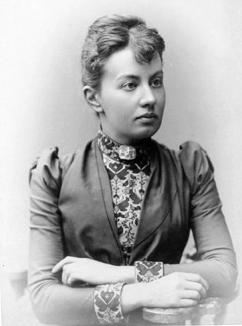
\includegraphics[width=0.25\textwidth]{kovalevskaya_8}
\end{wrapfigure}

Sofya Vasilyevna Kovalevskaya (1850-1891) è stata una matematica russa. Per varie ragioni, tra cui proprio il teorema al centro di questa discussione, è tuttora una delle figure femminili più rilevanti per la storia di questa disciplina.

Prima di tutto, è importante sottolineare che, da qui in poi, ci riferiremo spesso a lei con il nome con cui soleva firmarsi nelle sue pubblicazioni, ovvero Kowalevski.

Per allontanarsi dalla Russia dovette prendere parte a un matrimonio bianco, difatti sposò un uomo con cui, per diversi anni, non ebbe alcun reale rapporto sentimentale e da cui rimase spesso anche geograficamente distante.
Tutto ciò le permise di continuare a studiare in Germania; ed è qui che conobbe Karl Weierstrass, uno dei matematici più influenti del suo tempo.
Dopo una prima conoscenza avvenuta nello studio del professore, il rapporto tra loro continuò a svilupparsi grazie alle evidenti doti matematiche di Kowalevski, che Weierstrass non poté fare a meno di assecondare. Infatti, continuò a impartirle lezioni private, fino ad arrivare a supervisionare il suo lavoro di ricerca.

Per quanto riguarda le idee politiche di Kowalevski, possiamo affermare, con certezza storica, la sua vicinanza a movimenti femministi e idee socialiste e radicali, le quali possono essere fatte risalire al suo background familiare e agli spunti che colse durante la sua esperienza di vita negli stati dell'odierna Europa. È certamente degno di nota il fatto che ricevette in regalo da Anna, sua sorella, diverse copie di riviste radicali di quel tempo, le quali discutevano del cosiddetto nichilismo russo\footnote{la scienza, e non la religione o la superstizione, veniva considerata dai nichilisti russi come il mezzo più efficace per aiutare la popolazione a condurre una vita migliore e rappresentava, quindi, verità e progresso}.

Quello su cui vogliamo concentrare la nostra attenzione non sono le sue idee politiche, sociali e filosofiche, ma piuttosto il contributo che apportò alla matematica. Kowalevski, con l'aiuto di quello che possiamo chiamare il suo mentore, arrivò a diverse scoperte importanti. Dopo diversi anni di collaborazione, pubblicò ben tre tesi di dottorato in un solo anno: il 1874. Ma questo non è l'unico aspetto notevole, infatti, fu anche la prima donna a conseguire un dottorato, anche grazie al supporto di Weierstrass, come emerge da una lettera che scrisse lui stesso a Fuchs, un suo collega all'Università di Berlino, a riguardo dell'approvazione delle tesi di Kowalevski. Inoltre le sue pubblicazioni, oltre che significative per quanto appena detto, si rivelarono delle pietre miliari della matematica. In particolare i temi trattati sono:
\begin{itemize}
\item Equazioni differenziali alle derivate parziali (EDP), teorema di Cauchy-Kowalevski
\item Meccanica, Kowalevski top
\item Integrali ellittici
\end{itemize}


Dopo il successo, coronato anche da alcuni premi, che naturalmente seguì alla pubblicazione di queste ricerche, ritornò per un periodo in Russia; scelta che però si rivelerà di fatto inutile per il proseguimento della sua carriera accademica. Successivamente, quando il marito a cui doveva l'opportunità di aver studiato in Germania venne a mancare, si trasferì in Svezia, dove collezionò un altro primato: divenne la prima donna al mondo professoressa di matematica, ottenendo una cattedra all'Università di Stoccolma.
Purtroppo la sua vita venne interrotta prematuramente all'età di 41 anni da una polmonite, che, considerando quanto emerge dalle fonti, le impedì di portare avanti una sua grande passione: la produzione letteraria.
Nonostante, in quest'ambito, non abbia potuto esprimersi come avrebbe voluto, esistono numerose sue rappresentazioni artistiche, sia in letteratura che nel cinema.

Citiamo di seguito le opere cinematografiche principali:
\begin{itemize}
\emergencystretch 3em
\item \textit{Sofya Kowalevski}(1985, Lenfilm, 3 episodi, 218 minuti), Ayan Gasanovna Shakhmaliyeva (1932-1999,
originaria dell'Azerbaijan).

\item \textit{A Hill on the Dark Side of the Moon} (Svedese: \textit{Berget på månens baksida})(1983), Lennart Hjulström (1938-2022)
\end{itemize}

Citiamo di seguito le opere letterarie principali:
\begin{itemize}

\item una biografia: \textit{Sonja Kovalevsky. Ciò che ho vissuto con lei e ciò che mi ha detto di sé} (1892, Ed. Albert
Bonniers, Stoccolma), Anne Charlotte Leffler (una cara amica di Kowalevski sorella del matematico Gösta Mittag-Leffler e moglie dell'algebrista italiano Pasquale del Pezzo)

\item un'autobiografia: \textit{A Russian Childhood} (1978, Springer New York, NY), Sofya Kovalevskaya, tradotto e curato da Beatrice Stillman

\item una biografia: \textit{Little Sparrow: A Portrait of Sophia Kovalevsky} (1983,
Ohio University Press, Athens, Ohio), Don H. Kennedy

\item un romanzo biografico: \textit{Beyond the Limit: The Dream of Sofya Kovalevskaya} (2002, Tom
Doherty Associates, LLC), Joan Spicci (matematico ed educatore)

\item un racconto biografico: \textit{Too Much Happiness}\footnote{ il racconto ripercorre gli ultimi giorni di vita di Kowalevski arricchito da reminiscenze del passato
che Munro ha acquisito da lettere, diari e scritti (documenti a cui ha potuto
accedere tramite la moglie di Don H. Kennedy la quale è una lontana discendente di Kowlevski)} 
(2009, Harper's Magazine), Alice Munro (1931-2024, premio Nobel per la letteratura)

\end{itemize}

\section{Il teorema di Cauchy-Kowalevski}\label{introck}

Una volta introdotta la figura storica, possiamo ora fare il primo passo verso la scoperta di una delle ricerche di Kowalevski: il teorema di Cauchy-Kowalevski, che da qui in poi capiterà di abbreviare con l'acronimo TCK.

\emergencystretch 3em
Innanzitutto, descriviamo rapidamente il contesto scientifico di quel tempo relativo all'ambito delle EDP. 

Padre di queste ricerche che si svolgevano nell'Ottocento è Augustin-Louis Cauchy, un matematico che sarà sicuramente noto al lettore. In quegli anni, in particolare tra il 1835 e il 1842, Cauchy si stava occupando di sviluppare la teoria delle funzioni olomorfe, già avviata da altre grandi personalità di spicco come Eulero, Laplace e Fourier.

Cauchy ebbe l'intuizione di applicare questi risultati alle equazioni differenziali. 

Quello che è importante cogliere, cercando di calarsi nella mentalità di quel periodo, è che la teoria classica e le serie di potenze erano strumenti molto promettenti, in primis per la loro semplicità ed eleganza, ma anche per la potenzialità di approssimazione che racchiudeva un semplice troncamento di una serie.

Il tentativo di Cauchy di applicare alle equazioni differenziali gli strumenti ottenuti dalle sue ricerche fu un successo, ma si rivelò soltanto parziale per una semplice ragione: egli non riuscì ad andare oltre lo studio di equazioni differenziali ordinarie (EDO) e di EDP lineari.

Il salto avvenne proprio grazie a Kowalevski e Weierstrass. Quest'ultimo fu molto ottimista sui risultati che pensava si potessero raggiungere, forse ancora più di Cauchy: basti pensare che enunciò una congettura secondo la quale sarebbe stato possibile definire funzioni analitiche tramite equazioni differenziali, grazie a serie di potenze formali ricavate dalle espressioni delle equazioni.
Per tale ragione, spinse Kowalevski, insieme al suo talento, verso questo tema, nel quale lei seppe indagare molto più a fondo.

È sbagliato, però, pensare che le guide di Kowalevski furono soltanto Cauchy e Weierstrass: altri matematici si dedicarono a queste tematiche, tra i quali ricordiamo, tra i più importanti, Briot, Bouquet e Fuchs, che svilupparono meglio i concetti di singolarità, e Jacobi, che fornì per primo la definizione di equazione in forma normale\footnote{questo, in particolare, si rivelerà un concetto cruciale nella ricerca di Kowalevski}.

Da queste basi, l’idea importante avuta da Kowalevski può essere riassunta in questo modo: 
\begin{enumerate}
\item attuare un cambio di variabile che permettesse di scrivere un'equazione non-lineare in forma normale (si vedano i capitoli \ref{tools} e \ref{invariant} per il significato di questo termine), mantenendo le ipotesi di regolarità sui dati, e di potersi occupare dell’esistenza di una soluzione a questo sistema;
\item trasformare un'equazione qualsiasi in forma normale in un sistema quasi-lineare particolare;
\item applicare a tale sistema il metodo dei maggioranti già utilizzato da Cauchy per le sue scoperte su EDO ed EDP lineari.
\end{enumerate}

\newpage
Come accade spesso in matematica, la dimostrazione venne poi semplificata da E. Goursat in un suo libro di testo di analisi matematica risalente al 1900 circa. Inoltre, nel corso del tempo, vennero proposti enunciati e dimostrazioni più astratti e più generali, grazie al lavoro di Ovsyannikov, Treves e Nirenberg.

Notiamo rapidamente che, nello stesso periodo, anche Darboux raggiunse risultati molto simili a Kowalevski, ma con meno generalità.

Alla luce di quanto detto fino ad ora, ci poniamo alcune domande cruciali, a cui vogliamo trovare risposte quanto più esaustive possibile e che ci guideranno nel discorso che affronteremo:
\begin{itemize}
\item è possibile che esista una soluzione analitica a un sistema di EDP con dati di Cauchy?
\end{itemize}
in caso affermativo
\begin{itemize}
\item sotto quali ipotesi?
\item la soluzione è unica?
\item la soluzione dipende con continuità dai dati?
\item quali conseguenze e applicazioni hanno i risultati ottenuti?
\end{itemize}



